\documentclass[11pt]{article}
\usepackage{amsmath,textcomp,amssymb,geometry,graphicx,tikz,cancel,caption}
\usepackage{algpseudocode,algorithm}
\usepackage[colorlinks=true,urlcolor=blue]{hyperref}
\usepackage[T1]{fontenc}

\def\Name{Zack Field, Tohma Judge, Steve Hoffman, Andy Cheon}  % Your name
\def\Session{Spring 2014}

\title{LNC: Graph Theory Rough Draft}
\author{\Name}%, \texttt{\Login}}
\markboth{BIOEC144 --\Session\  \Name}
{BIOEC144 --\Session\ \Name}%, \texttt{\Login}}
\pagestyle{myheadings}

\begin{document}
\maketitle


\begin{tabular}{| l | l | p{6cm} |}
\hline
{\bf Name} & {\bf Expertise} & {\bf Contribution} \\ \hline 
Andy Cheon & BioE/bioinfo/programming & Glossary \& Test Quesions \\ \hline
Tohma Judge & BioE & External Resources \& Commentary \\ \hline
Steve Hoffman & Genetics/Biochem & Overview: Life Sciences \\ \hline
Zack Field & BioE/EECS & Overview: Math/CS/Engineering \& Graph Theory papers \\ \hline
\end{tabular}


\section*{WHAT IS A GRAPH? (by everyone)}  

\begin{figure}
        \centering
        \begin{subfigure}{\textwidth}
                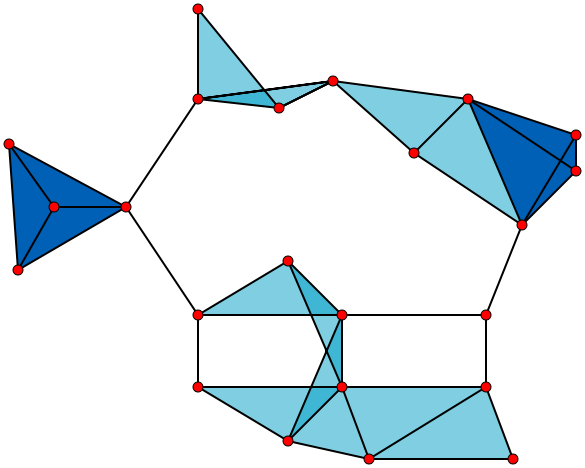
\includegraphics[width=0.4\textwidth]{clique.png}
                \label{fig:clique}
        \end{subfigure}%
         ~ %add desired spacing between images, e. g. ~, \quad, \qquad etc.
          %(or a blank line to force the subfigure onto a new line)
        \begin{subfigure}{\textwidth}
                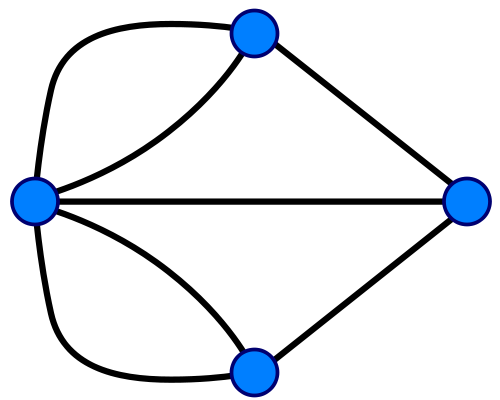
\includegraphics[width=0.4\textwidth]{konig7.png}
                \label{fig:konig}
        \end{subfigure}
        \caption{Examples of graphs}\label{fig:graphs}
\end{figure}


{\bf Graphs} are composed of {\bf nodes}({\bf vertices}) and edges. {\bf Edges} connect vertices, 
and can have a {\bf direction} and a {\bf weight}. {\bf Degree}, or {\bf valency}, 
is the number of edges connected to a node. 
If direction is being used in the graph, count two separate degrees, 
one for away from the node and one for into the node. 
A {\bf complete graph} has all its nodes connected by an edge to each other. 
They are noted as $K_{n}$, where n is the number of nodes. 
A {\bf clique} is a set of vertices in a graph that forms a complete graph. 
A {\bf hub} is a node connected to a large number of nodes.

There are many everyday-life representations of graphs.  
Highways linking together cities, for example, are the edges of a directed graph.  
Vary the speed limit or the number of cars on each highway, and that graph 
becomes weighted.

\section*{OVERVIEW -- MATH / CS / ENGINEERING}

Graphs can be used wherever there is an interest in analyzing pairwise information. 
Graph theory is a mature field, and our understanding of the structure of, 
and information contained in, graphs is vast (although far from complete). 
As computational biologists we can use this accumulated knowledge of graphs to 
our advantage when analyzing data and attempting glean meaningful relationships 
within a dataset. A reliable strategy is to represent elements (objects) in 
your data as {\bf vertices} and the relationships between them as {\bf edges}. 
The ability to construct these graph relies on knowledge of biology, and intuition. 
This abstraction of relationships in data to a graph allows for formal analysis of the problem. 
After a graphical representation is formulated, the next step is to find some kind of structure 
(or particular element) within the graph (e.g. maximal clique, minimum pairwise distance, maximum flow). 
The graphical representation of your data will be based on the type of problem that you are trying to solve, 
and the structure you wish to find. 

The complexity (difficulty) of your problem will follow from the structure or element 
that you are trying to uncover. 
An example (from lecture): The homology of proteins. We know that hierarchical clustering 
is used in conjunction with pairwise comparisons of proteins (by MDL or other methods). 
How could that problem be represented as a graph? We could start by placing the 
proteins at each of the {\bf vertices}. The {\bf edges} between each vertex would have a 
weight determined by pairwise alignment. This is an abstract enough definition of 
the problem that any decent general hierarchical clustering algorithm would return 
a hierarchy of clusters. If the pairwise alignment method is positively correlated with the 
homology of two proteins, then this hierarchy would be equivalent to a phylogenetic tree. 

We can use hierarchical clustering as an example to see how the complexity of the problem 
relates to the structure or element that we wish to uncover. 
Each iteration of hierarchical clustering seeks to find the two elements that are most 
closely related (smallest weight edge). This means that for $n$ vertices (proteins) we have to 
check $n^2$ edges (alignment scores) to find the smallest. 
Since one edge is removed with each iteration, our total running time is $O(n^3)$. 
Unfortunately, many of the interesting problems in graph theory, and (graph theoretic formulations of problems in biology) 
are not solvable in polynomial time. Many problems take exponential time in the size of their input: $n$ “proteins” $O(c^n), c>1$ 
(i.e. NP-complete problems). 
If formulated in the right way, most problems in biology can be reduced to problems 
already discovered in the theory of graphs and related fields. 
It is up to computational biologists to provide the insight necessary to make 
these reductions. 

\section*{OVERVIEW -- LIFE SCIENCES}

To familiarize individuals with graph theory with little computational background, 
this section will present the practical application of graphs in biology with examples. 
Graphs are fundamental in understanding in vivo interactions between molecules. 
Protein-protein interaction (PPI) networks, regulatory networks (GRNs) which 
contain information regarding gene expression, signal transduction networks, and 
multiple integrated metabolic pathways are examples requiring the use of graph theory. 
Any pathway you learned in biochemistry could be demonstrated by a graph.

Consider the following graphic that displays blood clotting in vivo induced by trauma:

\begin{figure}
  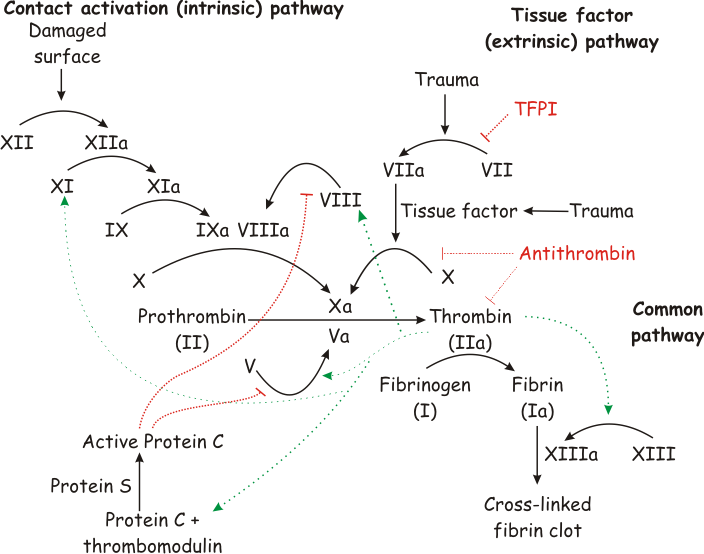
\includegraphics[width= 0.8\textwidth]{graph-bio.png}
  \label{fig:graph-bio}
  \caption{Graph representation of blood clotting process}
\end{figure}

This heavily regulated pathway involves a multitude of proteins activating (dotted lines with arrows) and 
inhibiting (dotted lines with flat line) others. 
Such interactions could be represented as edges on a graph, 
with the proteins represented as nodes.
If we have a well-formed graph and consider that many problems in graph theory 
are well characterized, is there still be a need for biologists in 
computational biology? Absolutely. 
If you gave a computer scientist who has no background in basic principles of 
biology several protein sequences, they would not know what biochemical information 
is relevant in constructing a graph. In the context of PPI networks, 
knowing the interactions between proteins underscores the need for biologists 
in endeavors in computational biology. A computer could predict PPI networks but 
there could be false positives that predict interactions between proteins when 
there should not. Such a lack of an interaction could be demonstrated by a biologist 
in a laboratory. 

\section*{GRAPH THEORY PAPERS}

\begin{itemize}
\item (intro) \href{http://www.youtube.com/watch?v=HmQR8Xy9DeM}{Graph Theory introduction video}
\item (intro) \href{http://home.deib.polimi.it/matteucc/Clustering/tutorial_html/hierarchical.html}{Hierarchical Clustering Explanation}
\item (intermediate) \href{http://www.hamilton.ie/systemsbiology/files/2006/graph_theory_and_networks_in_biology.pdf}{Graph Theory and Networks in Biology}
\item (intermediate) \href{http://www.ncbi.nlm.nih.gov/pmc/articles/PMC3101653/}{Using graph theory to analyze biological networks}
\item (advanced) \href{http://www.cs.berkeley.edu/~vazirani/algorithms/}{Berkeley's canonical algorithms text: "Algorithms"} (recommend Ch. 3 & Ch. 4)
\item (advanced) \href{http://code.google.com/p/graphbook/}{(another) Graph theory text}
\end{itemize}

\section*{COMMENTARY}

Cs Foundations Short 2014
Slides 28-36
	
Graphs are composed of nodes(vertices) and edges. Edges connect vertices, and can have a direction and a weight. Degree, or Valency, is the number of edges connected to a node. If direction is being used in the graph, count two separate degrees, one for away from the node and one for into the node. A Complete Graph has all its nodes connected by an edge to each other. They are noted as Kn, where n is the number of nodes. A Clique is a set of vertices in a graph that forms a complete graph. A Hub is a node connected to a large number of nodes.

Graphs are useful for storing and analyzing interaction data, using programs such as Cytoscape. Examples of Graph usage given include a KEGG(Kyoto Encyclopedia of Genes and Genomes) pathway, where nodes represent substrates, while edges represent enzymatic reactions; Whole-Genome interactomes, where nodes represent Protein-Protein Interactions. Certain patterns become easy to spot when using graphs-a protein with many interactions will appear as the hub of a large network. Anything that can be represented as a node with connecting edges is graphical in nature. Some examples below 

\begin{tabular}{| l | l | l |}
\hline
Example & Node represents & Edge represents \\ \hline
KEGG PAthway & Substrate & Enzymamtic Reactions \\ \hline
Whole-Genome Interactomes & Proteins & Protein-Protein interation (PPI) \\ \hline
Love Triangle & Person & Attraction (directed!) \\ \hline
Phylogenetic Trees & Species & Relation \\ \hline
\end{tabular}
\section*{EXTERNAL RESOURCES / LINKS}

\begin{itemize}
\item "protein-protein interaction networks and biology--what's the connection?" hakes et al nature biotechnology 2008. Recommended by slide, unsure if this counts under third party or would go under assigned reading/recommended?
\item A quick excerpt from a text on transportation networks, but clearly defines basic terms for graph theory.
\href{http://people.hofstra.edu/geotrans/eng/methods/ch1m2en.html}{Graph Theory terms}
\item \href{http://www.doc.ic.ac.uk/~natasha/book_chpt5_GT_NP.pdf}{Review of Graph Theory in relation to proteomics}. 
Covers terminology, biological terminology such as pathways and homology and their adaptation to graph data structure, Network properties such as clustering within a graph, describes random graphs, small networks, and scale free networks. The next section describes PPI data collection, and defines pathways. Lastly, it goes over properties of PPI networks constructed from said data and other notes for analysis. Should be noted that this is a fairly large paper, hitting nearly 61 pages. 
Unknown if this is too large for the LNC
\item \href{http://bix.ucsd.edu/bioalgorithms/presentations/Ch08_GraphsDNAseq.pdf}{Presentation on graph theory's application to early genetic sequencing problems},
goes over Euler theorem and it's application to sequencing by hybridization. 
Very good examples of graph theory being applied to problems that don't 
immediately appear to involve graphical information.
\item \href{http://bix.ucsd.edu/bioalgorithms/presentations/Ch08_GraphsDNAseq.pdf}{Powerpoint going over graph theory}, 
  very clear description of the possible computational representations of a graph, 
  as well as some applicable algorithms, such as dijkstra. 
  Definitely nice for looking at graph theory from an entirely computation based perspective.
\end{itemize}

\section*{COMPREHENSION TEST QUESTIONS}

\begin{enumerate}
\item Categorize the graph below as 
  \begin{itemize}
  \item[(a)] directed or undirected
  \item [(b)] cyclic or acyclic
  \item [(c)] complete or incomplete
  \item [(d)] weighted or unweighted
  \end{itemize}
  What are the shortest and longest paths from node A to node E?  
  
  List any cliques you find.

  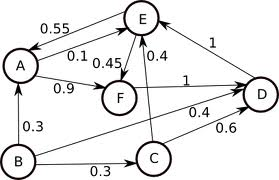
\includegraphics[scale=0.5]{q1.png}

\item What might the graph of a signaling pathway look like?  
  Categorize the graph as you would in (1).

\item What might be some of the advantages and disadvantages of modeling biological systems with graphs?
\end{enumerate}


\section*{GLOSSARY}

\begin{tabular}{| l | p{5cm} | p{4cm} | p{4cm} |}
\hline
Term & Definition & Notes/Comments & Related Words\\ \hline
acyclic graph & a graph where no possible cycles are present; i.e. following any path will not lead to a node that was already visited && opposite: cyclic graph \\ \hline

clique & a set of vertices in a graph that forms a complete graph && \\ \hline


complete graph & a graph that has all its nodes connected by an edge to each other && opposite: incomplete graph \\ \hline

cyclic graph & a graph where one or more possible cycles are present; i.e. following any path could lead to a node that was already visited && opposite: acyclic graph \\ \hline

directed graph & a graph in which edges have direction & Edges of a directed graph are represented with arrows & opposite: undirected graph \\ \hline

edge & a connection that links two vertices & may or may not be directional & \\ \hline

hub & a node connected to a large number of nodes && \\ \hline

incomplete graph & a graph that does not have all its nodes connected by an edge to each other && opposite: complete graph \\ \hline

indegree & the number of edges entering a vertex && opposite: outdegree \\ \hline 

node & a point on a graph; may be connected to other nodes by edges or may be isolated && a.k.a. vertex \\ \hline

outdegree & the number of edges leaving a vertex && \\ \hline

undirected graph & a graph in which edges do not have direction && opposite: directed graph \\ \hline

valency & number of edges connected to a node && \\ \hline

vertex & a point on a graph; may be connected to other nodes by edges or may be isolated && a.k.a. node \\ \hline

weight & a level of "importance" or "heaviness" assigned to an edge e.g. distances of highways linking cities, or closeness between friends on a social network & a graph with weights is known as a weighted graph & \\ \hline

\end{tabular}





\end{document}
